\chapter{Neural Networks}

{\sf An inspiration to a neural networks mashines comes from biological neural networks. In 1950's we already knew how it works. The the main thing that allows a neuron to filter all the useless signals that happend in the brain all the time is all-or-none law: if a signal exceeds the threshold potential, the neuron will give a complete response; otherwise, there is no response.}

\section{Perceptron}

So the perceptron works the same. However, it can be represented as the small neural network where input neurons are the signals what multiplied by some coefficients, then all results add up and if sum is over some threshold, we get the signal $+1$, otherwise, we get $-1$. The problem with that is we can only have one layer: if you combine several layers as how it happens in the brain, you will have no good way of training the multi-layer perceptron with the simple threshold function. So the way around it is replace the threshold function for something more complex. The first aproach is a single layer neural network with logistic function as a threshold.

\section{Single Layer Networks}

The single layer neural network with logistic function is called logistic regression. The logistic regression is the classification algorithm, not the regression algorithm. It's just called like that.

\subsubsection*{Logistic regression}

For the binary classification (with classes $+1$ and $-1$) the math comes out very nicely; the probability of the signal is the one minus the probability of the reverse signal:
$$P(y|x)=\begin{cases}
f(x)&\text{for }y=+1,\\
1-f(x)&\text{for }y=-1.
\end{cases}$$
This sigmoid function $\sigma$ satisfies the both parameters of $P(x|y)$:
$$P(y|x)=\sigma(yw^Tx),\qquad\sigma(s)=\frac{1}{1+e^{-s}},\qquad \sigma(s)=1-\sigma(s)$$
where $w^Tx$ is the answer of the perceptron in input $x$.\\
So if our output is the probability of classes, how would we calculate the loss function? How we would calculate the error what we can try to minimize? Well, we just use likelyhood:
$$\prod\limits_{i=1}^{N}P(y_i|x_i)=\prod\limits_{i=1}^{N}\sigma(y_iw^Tx_i)$$
Then we go from multiplication to sum of the logarithms and get loss function (what we will try to minimize) for the logistic regression:
$$L(w)=-\frac{1}{N}\ln\left(\prod\limits_{i=1}^N\sigma(y_iw^Tx_i)\right)=\frac{1}{N}\sum\limits_{i=1}^N\ln(1+e^{-y_iw^Tx_i})$$

Now the problem is training it. Even for one layer logistic regression we need to utilise the gradient descent:
$$w(t+1)=w(t)-\eta\frac{\partial C(w)}{\partial w}$$
The $C(w)$ is the cost function (instead it we can the use loss function; we typically talk about the loss function $L(w)$ (or $J(w)$) and the cost function $C(w)$). And we have the learning rate $\eta$.\\
In case of large data it becomes hard to calculate the average value of all logarithms in the loss function $L(w)$. However, we can go around by using a stochastic gradient descent: just calculate the loss function for batch (some part of the data) and then apply the gradient descent step for that batch. So if we use the stochastic gradient descent, at first we need to split our data into random batches and complete the gradient descent step for every batch. This iteration is called an epoch. The number of steps in one epoch is number of all points divided by the size of the betch ($N / N_{batch}$).
So this is the difference beteen the gradient descent and stochastic gradient descent:
$$\text{Gradient Descent: }w\leftarrow w-\eta\left(-\frac{1}{N}\sum\limits_{i=1}^N\frac{y_ix_i}{1+e^{y_iw^Tx_i}}\right)$$
$$\text{Stochastic Gradient Descent: }w\leftarrow w-\eta\left(-\frac{1}{N_{batch}}\sum\limits_{x_i\in batch}\frac{y_ix_i}{1+e^{y_iw^Tx_i}}\right)$$
Also we have a very stochastic gradient descent (when every bench contains only one point).\\
%$$w\leftarrow w-\eta\frac{\partial C(w^Tx_i,y_i)}{\partial w}$$
{\it <The reason why very stochastic gradient descent is not the best way>}

\section{Several Layers Networks}

So we have the algorithm for training in one layer neural network. The way to trainig the several layers is the back-propagation. 

\subsubsection*{Back-propagation}

At first we need to define some coefficients and numbers:
\begin{enumerate}[label=$\bullet$]
  \item $w_{jk}^l$ is the weight between neuron $j$ in layer $l-1$ and neuron $k$ in layer $l$.
  \item $x_j^l$ is the outcoming signal after the activation function, i.e. $x_j^l=\sigma\left(\sum w_{ij}^lx_i^{l-1}\right)$ (for the logistic regression $\sigma$ is the sigmoid function). In the first layer $x_j^1=x_j$ ($x_j$ is a feature). You can look at all $x_i^l$ in other layers at the features as well (sometimes they called feature layers).
  \item $s_j^l$ is the incoming signal to neuron $j$ in layer $l$, $s_j^l=\sum w_{ij}^lx_i^{l-1}$
\end{enumerate}
So the values what we try to optimise is $w$'s. We want to calculate the gradient for loss functions over the $w$'s. This is the goldest way to calculate the partial derilivative of our loss function:
$$\nabla C_{w_{ij}^l}(w)=\frac{\partial C(w)}{\partial w_{ij}^l}=\frac{\partial C(w)}{\partial s_j^l}\times\frac{\partial s_j^l}{\partial w_{ij}^l}$$
Also we have
$$\frac{\partial s_j^l}{\partial w_{ij}^l}=x_i^{l-1}$$
because $s_j^l=\sum w_{ij}^lx_i^{l-1}$. Then we calculate $\delta_j^{l-1}$ what is defined as
$$\delta_j^{l-1}=\frac{\partial C(w)}{\partial s_j^{l-1}}$$
If the loss function $f$ is diferantionable then we just calculate all partial derilivatives for the last layer $L$:
$$\delta_i^L=\frac{\partial C(w)}{\partial s_i^L},\qquad C(w)=f(x^L),\qquad x_i^L=\sigma(s_i^L)$$
For the previous layers we can again apply the chain rule and calculate the $\delta_i^{l-1}$ using $\delta_i^l$:
$$\delta_i^{l-1}=\frac{\partial C(w)}{\partial s_i^{l-1}}=\sum\limits_{j}\frac{\partial C(w)}{\partial s_j^l}\times\frac{\partial s_j^l}{\partial x_i^{l-1}}\times\frac{\partial x_i^{l-1}}{\partial s_i^{l-1}}=\sum\limits_{j}\delta_j^l\times w_{ij}^l\times\sigma'(s_i^{l-1})$$
So back-propagation algorithm looks like this:
\begin{enumerate}[label=\arabic*.]
  \item Initialize weights randomly (with small random numbers in $[-0.1,0.1]$).
  \item Compute the forward path: calculate all $x$ and $s$.
  \item Go backward and calculate all $\delta$.
  \item Shift all weights: $w_{ij}^l\leftarrow w_{ij}^l-\eta x_i^{l-1}\delta_j^l$ ($\eta$ is some learning rate).
  \item Go to step 2.
\end{enumerate}
The important thing is you can calclulate all $\delta$ with tensors: you don't have to iterate over each coefficient but rather multiply tensors. Which is good because we can push it into the GPU's what are really good in multiplying thensors.

\subsubsection*{Activation functions}

Sigmoid: 
$$\sigma(s)=\frac{1}{1+e^{-s}}$$
Tanh:
$$\sigma(s)=\frac{e^s-e^{-s}}{e^s+e^{-s}}$$
Rectified Linear Unit (ReLU):
$$\sigma(s)=\max(0,s)$$
The sigmoid finction goes from 0 to 1. If you want something what can be negative you can use hyperbolic tangent what goes from $-1$ to 1. And if you want something what calculates very fast and doesn't get your gradient diminished when you reach big numbers you can use ReLU.

\subsubsection*{Softmax and cross-entropy}

In case of binary classification you use logistic function and you have one output neuron what gets the probability of one class. In multiclass classification case we utilize the function what is called the Softmax:
$$x_j^L=\sigma^L(s_j^L)=\frac{e^{s_j^L}}{\sum e^{s_i^L}}$$
It is called Softmax because all last layer neurons output numbers around 0 (exept one that outputs number around 1).\\
The cross-entropy loss function is:
$$C(w)=\sum o_i\log(x_i^L),\qquad o_i=\begin{cases}
1&\text{if }y=i,\\
0&\text{if }y\ne i.
\end{cases}$$
{<\it Some talk what I can't understand>}\\
The networks what are orginised like that is called fully conected network: each neuron of the one layer connects with each neuron of the next layer and so on.

\section{Regularization}

Networks, espesualy fully conected, are very prompt to overfitting. For example let's say we have a very big network and train it to recognize images. Instead of learning features of the images, for example, recognizing a cat from a car by ears and so on, big neural networks can just memorize the images: it can looks on the value of concrete pixel. This is an overfitting -- memorising the dataset,  noise training and so on. How we can to regularize it? 

\subsubsection*{L2 regularization}

When we regularize we trying to lower the VC-dimention, lower the number of possible hypotheses. We do that by adding some constraints to the loss function. Here we add the L2 constraint:
$$C_{new}(w)=C(w)+\frac{\lambda}{2N}\|w\|_2^2$$
This way is called the L2 regularization or weight decay.\\
{\it <Some intuition why it works>} %If you look at the derilivative of the funсtion $C_{new}$ you will have derilivative of the loss function $C(w)$ and the negative weight. <...>

\subsubsection*{Early stopping}

\begin{wrapfigure}{r}{0.4\linewidth}
  \vspace{-1.3cm}
  \begin{center}
    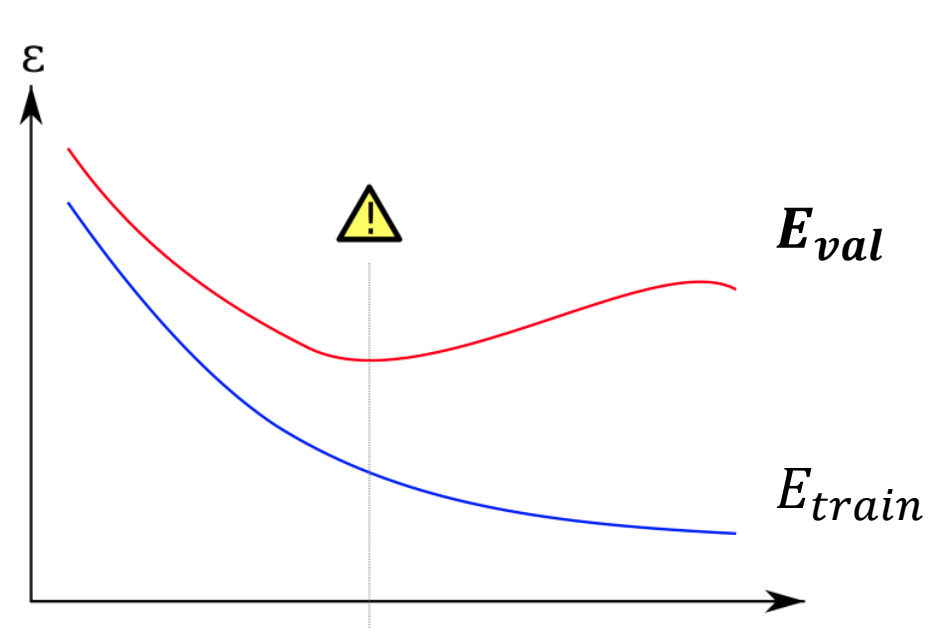
\includegraphics[width=\linewidth]{6a.png}
  \end{center}
  \vspace{-0.3cm}
  \caption*{(6.1) Early stopping}
  \vspace{-1.5cm}
\end{wrapfigure}
The another way in regularization is catching the moment of overfitting. So this is a typical graph [pic.~6.1] what shows gain between errors on the validation dataset and training dataset (the x axis is the number of epochs).\\
The error on the training dataset is always decrease, but error in the validation dataset in some point starts to increase. And at that point we want to stop (remember the weights of the network in that point).

\subsubsection*{Dropout}

Dropout is a direct way to preventing networks from memorizing the dataset. We just turn of some (50\%, for example) random neurons for every layers in every patch. The turned of neuron outputs 0. In that way the network will try to learn general features rather than specific pathways, because each pathway can be turned off.\\
\begin{figure}[h!]
  \centering
  \begin{subfigure}[l]{0.3\linewidth}
    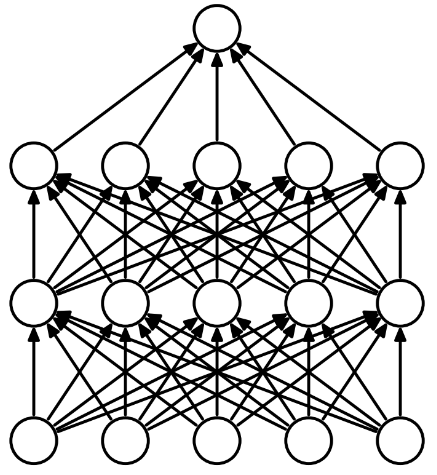
\includegraphics[width=\linewidth]{6b.png}
    \caption*{(6.2) Standart neural net}
  \end{subfigure}
  \hspace{2cm}
  \begin{subfigure}[r]{0.3\linewidth}
    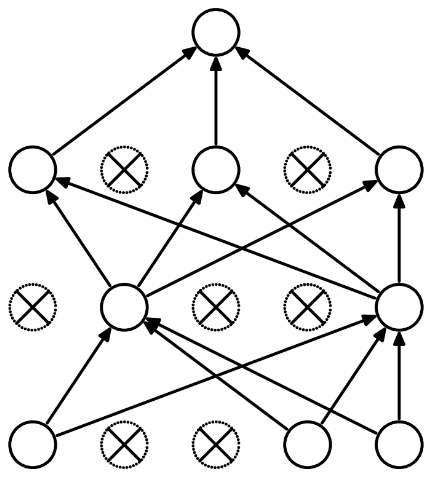
\includegraphics[width=\linewidth]{6c.png}
    \caption*{(6.3) After applying dropout}
  \end{subfigure}
\end{figure}
When we apply this network at some task we need to turn on all the neurons.

\subsubsection*{Data augmentation}

The overfitting doesn't happen if you have a lot of data. How to create a lot of data we will talk at the next lecture.

\section{Deep Learning Libraries}

If you don't like Python, learn to like Python because most of deep learning done in it. However there is still some inthusiasts what work on the deep learning for Java \href{http://deeplearning4j.org/}{library}.\\
Google represents \href{www.tensorflow.org}{TensorFlow} and the \href{keras.io}{Keras} (what is built on top of the first one). So if you just want to create networks simply you should use Keras. And if you want to create complex networks you should use TensorFlow.\\
The \href{torch.ch}{Torch} library easier than TensorFlow but more complex than Keras.